%!TEX root = main.tex

\chapter{Results and Analysis}

	This chapter discusses the quantitative and qualitative results of the testing from the several iterations. The analysis of the results and improvements made in accordance to those results are also discussed in this chapter.			

	\section{Universal Results}
		This section provides an overview of the universal results across all iterations. Note that questions for iteration 3 and 4 were different from that of iteration 1 and 2. Despite having different questions, all answers are on a scale of 1 - 4, 1 (Never, Strongly Disagree, or Very Difficult) being the lowest, and 4 (Frequently, Strongly Agree, or Very Easy) being the highest. 

		\subsection{Iteration 1} 

			\begin{table}[!htpb]
			  \centering
			  \captionof{table}{Feature Scores for Iteration 1} \label{tab:results-features-it1}
			  \begin{tabular}{|p{5cm}|R{.7cm}|R{.7cm}|R{.7cm}|R{.7cm}|R{.7cm}|R{1.5cm}|}
			  	\hline
			  	\textbf{Feature} & \textbf{T1} & \textbf{T2} & \textbf{T3} & \textbf{T4} & \textbf{T5} & \textbf{Average} \\ \hline
				Add a Note															& 3.0 & 2.3 & 2.5 & 3.3 & 3.0 & 2.8 \\ \hline 
				Edit a Note 															& 2.5 & 1.5 & 3.0 & 1.8 & 2.0 & 2.2 \\ \hline
				Delete a Note 														& 2.8 & 3.0 & 2.3 & 2.0 & 1.5 & 2.3 \\ \hline
				Move Indicator/Cursor 										& 3.0 & 3.8 & 3.3 & 4.0 & 4.0 & 3.6 \\ \hline
				Move Line/Space Selector 									& 3.3 & 2.5 & 2.8 & 4.0 & 4.0 & 3.3 \\ \hline
				Highlight/Select a Group of Notes 						& 2.8 & 2.5 & 3.3 & 2.5 & 1.3 & 2.5 \\ \hline
				Edit a Highlighted/Selected Group of Notes 		& 3.0 & 2.8 & 2.0 & 2.0 & 1.3 & 2.2 \\ \hline
				Delete a Highlighted/Selected Group of Notes 	& 3.0 & 2.5 & 3.3 & 1.0 & 1.0 & 2.2 \\ \hline
			  \end{tabular}
			\end{table}

			From the data gathered and analyzed, a clear difference in respondent sentiment was observed from features that needed note selection versus those that did not. This can be observed in the edit and delete features which had the lowest scores on average. Both of these features required the selection feature. Most of the respondents were not able to figure out and correctly execute the gesture for selection which was a two-finger drag. Although it is common for mobile applications to use one-finger drag to scroll, the results suggest otherwise. It was found that the gesture for highlighting (two-finger drag) would have felt more natural if it was switched with the scroll gesture (one-finger drag). Hence, for the second iteration, the gestures for these interactions were switched (see Figure \ref{fig:highlight}).

			\begin{figure}[h]
				\centering
				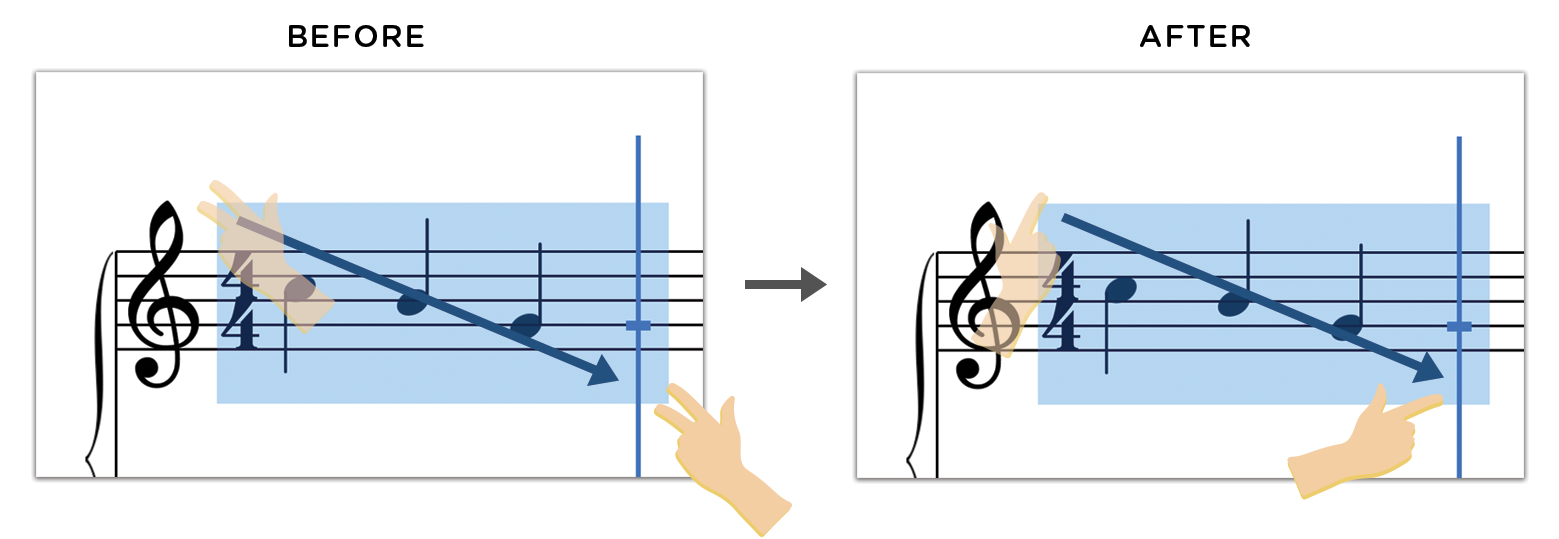
\includegraphics[scale=0.25]{figures/before-after-highlight}
			    \caption{The highlight interaction before and after changes were made due to the user testing. The new interaction uses only one (1) finger.}
			    \label{fig:highlight}
			\end{figure}

			Other than the note selection feature, respondents have expressed that most of the features worked well and felt comfortable to use. Although it was not like how they would regularly write music (i.e. pen and paper), Flow's method of composing was easy to learn and get used to. Majority liked the ease of using the cursor/indicator because they can simply tap on the location they want or use the arrow keys when they want to be accurate.

		\subsection{Iteration 2}
			\begin{longtable}{|p{5cm}|R{.7cm}|R{.7cm}|R{.7cm}|R{.7cm}|R{.7cm}|R{1.5cm}|}
			  \caption{Feature Scores for Iteration 2} \label{tab:results-features-it2} \\ 
			  	\hline
			  	\textbf{Feature} & \textbf{T1} & \textbf{T2} & \textbf{T3} & \textbf{T4} & \textbf{T5} & \textbf{Average} \\ \hline
				Add a Note 																							& 3.0 & 4.0 & 3.8 & 3.5 & 3.3 & 3.5 \\ \hline
				Delete a Note 																						& 3.5 & 1.8 & 4.0 & 2.5 & 4.0 & 3.2 \\ \hline
				Edit a Note 																							& 3.3 & 3.8 & 4.0 & 2.8 & 4.0 & 3.6 \\ \hline
				Move Position Indicator/Cursor 															& 3.8 & 3.0 & 4.0 & 3.3 & 3.8 & 3.6 \\ \hline
				Move Line/Space Selector 																	& 2.3 & 3.0 & 3.8 & 4.0 & 3.8 & 3.4 \\ \hline
				Highlight/Select a Group of Notes 														& 3.5 & 4.0 & 4.0 & 3.5 & 4.0 & 3.8 \\ \hline
				Edit a Highlighted/Selected Group of Notes 										& 4.0 & 1.8 & 4.0 & 4.0 & 4.0 & 3.6 \\ \hline
				Delete a Highlighted/Selected Group of Notes 									& 4.0 & 4.0 & 4.0 & 4.0 & 4.0 & 4.0 \\ \hline
				Scrolling																								& 3.3 & 3.8 & 3.5 & 3.0 & 3.8 & 3.5 \\ \hline
				Change Time Signature 																		& 3.3 & 1.8 & 3.5 & 3.5 & 3.8 & 3.2 \\ \hline
				Change Key Signature 																		& 3.5 & 4.0 & 3.0 & 3.0 & 4.0 & 3.5 \\ \hline
				Add an Accidental to a Note 																& 4.0 & 4.0 & 4.0 & 3.0 & 4.0 & 3.8 \\ \hline
				Remove an Accidental to a Note 														& 2.0 & 1.3 & 4.0 & 1.8 & 4.0 & 2.6 \\ \hline
				Zooming 																								& 3.3 & 3.3 & 4.0 & 3.0 & 4.0 & 3.5 \\ \hline
				Cut/Copy/Paste a Single Note 															& 4.0 & 2.0 & 4.0 & 1.0 & 4.0 & 3.0 \\ \hline
				Cut/Copy/Paste a Highlighted/Selected Group of Notes 					& 3.8 & 1.8 & 3.0 & 1.0 & 4.0 & 2.7 \\ \hline
				Select a Single Note 																			& 3.5 & 4.0 & 4.0 & 3.0 & 4.0 & 3.7 \\ \hline
				Add an Accidental to a Highlighted/Selected Group of Notes 			& 3.3 & 3.0 & 4.0 & 2.0 & 4.0 & 3.3 \\ \hline
				Remove an Accidental on a Highlighted/Selected Group of Notes 	& 2.0 & 2.5 & 3.0 & 2.0 & 4.0 & 2.7 \\ \hline
				Music Playback 																					& 4.0 & 4.0 & 4.0 & 4.0 & 4.0 & 4.0 \\ \hline
			\end{longtable}

			Iteration 2 added some design revisions incorporating the data from the results of iteration 1. The most notable change would be the completely different gesture interaction for highlighting multiple notes. This change resulted in a highlight interaction that not only uses less fingers, but is also less prone to errors. The new interaction influenced most of the results for features involving multiple note selection. Features that scored the lowest like \textit{Edit a Note} and \textit{Delete a Highlighted/Selected Group of Notes} in the first iteration scored higher for iteration 2 testers. \textit{Highlight/Select a Group of Notes} also scored the highest among the features that were also present in iteration 1. Testers were able to easily select multiple notes and access features that required note selection in iteration 2. 

			New features were also added in the iteration 2 testing. Given that it was only the first time these were tested, some scored low and were found to need improvement. An example would be the implementation of \textit{Change Time Signature} and \textit{Change Key Signature}. Both features were quite similar to each other because they utilized a slide interaction. However, the problem with sliders, especially the one for the time signature, was that they had a tendency to be imprecise. This was frustrating for the composers because just slight finger movements would already change the value. If they had a specific value in mind, they needed to be extremely precise and careful when setting the value. On the other hand, the key signature slider was easier, but it only showed a few values at a time so it was sometimes hard for them to find the key signature they wanted. For the succeeding iterations, the menu was changed to allow for easier changing of the time and key signature (see Figure \ref{fig:time-key-signature}).

			\begin{figure}[H]
				\centering
				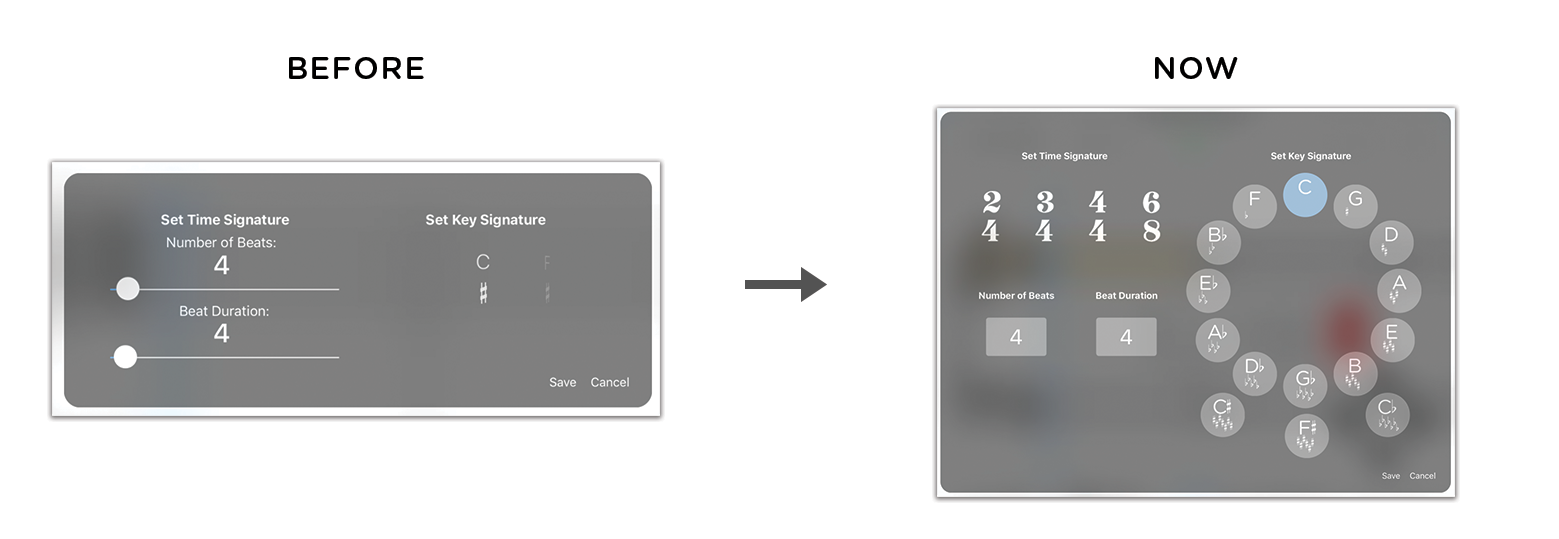
\includegraphics[scale=0.25]{figures/before-after-timesigmenu}
			    \caption{The time and key signature menu before and after changes were made due to the user testing. The revised time signature menu adds buttons for the common time signatures and also allows users to input any valid time signature they want. The revised key signature menu is now radial and follows the circle of fifths.}
			    \label{fig:time-key-signature}
			\end{figure} 

			The transposition interaction also needed improvement. In the iteration 1 and 2 prototype, users can tap on the up or down arrow keys to instantly transpose the selected notes to a higher or lower pitch respectively. It was observed that this was sometimes confusing and not easy to find. The confusion happened mainly because the users' assumption was that the arrow key was only used to move the cursor and not the notes. They would eventually be able to figure out after some messing around, but this still needed to be improved. Hence, in the succeeding iteration a menu was added containing the transpose arrow keys and other modifiers that would only appear when a user highlights a set of notes (see Figure \ref{fig:transpose}. This not only made it more obvious, but also saved space by only showing the necessary buttons when needed.

			\begin{figure}[h]
				\centering
				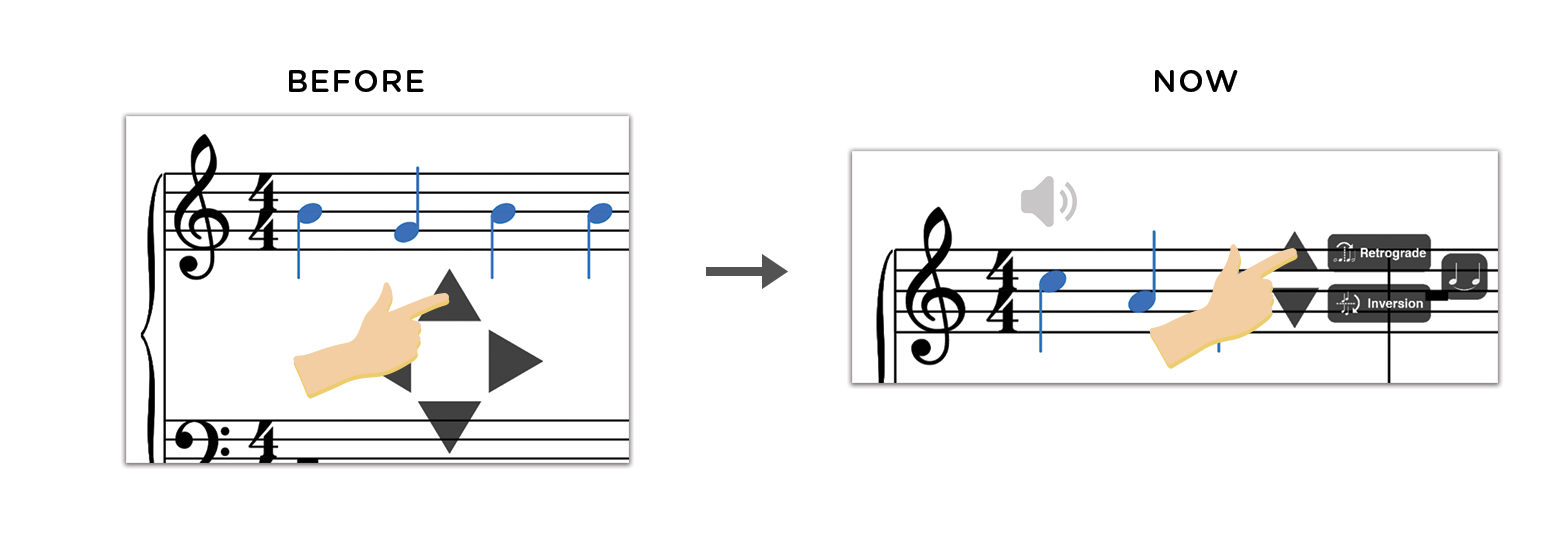
\includegraphics[scale=0.25]{figures/before-after-transpose-notes}
			    \caption{The transpose interaction before and after changes were made due to the user testing. The new transpose interaction adds a menu containing separate transpose arrow keys as well as additional modifiers.}
			    \label{fig:transpose}
			\end{figure}

			The feature that received the lowest score for this iteration was \textit{Remove an Accidental on a Highlighted/Selected Group of Notes}. A lot of the composers said they felt that the buttons were too small and hard to press. However, the main problem with the feature was that the buttons were set up to follow music theory. In music theory, when a sharp is added to a note, it needs to be naturalized to remove the sharp. This was also the logic behind the accidentals in the prototype. When a note has a sharp, the user would have to press the naturalize button to remove it. Unfortunately, this was not obvious to the amateur users. They expected it to be similar to making a text bold or italicized in word processors. What they commonly did was when a note had a sharp, they would press the sharp button again to remove it. Since the buttons were not set up to follow it, nothing would happen and they thought that the buttons did not work. Expert composers, however, did not have a problem using this feature. When asked why they were able to figure it out easily, they mentioned that they just followed music theory. To suit both types of users, the prototype in the succeeding iterations also allowed users to press the accidental button again to remove an already placed accidental aside from the original method of removing accidentals.

		\subsection{Iteration 3} % (fold)
		\label{sub:iteration_3}
		
			\begin{landscape}				
				\begin{longtable}{|p{3.5cm}|R{.7cm}|R{.7cm}|R{.7cm}|R{.7cm}|R{.7cm}|R{.7cm}|R{.7cm}|R{.7cm}|R{.7cm}|R{.7cm}|R{.7cm}|R{.7cm}|R{.7cm}|R{.7cm}|R{.7cm}|R{1.5cm}|}
					\caption{Feature Scores for Iteration 3} \label{tab:results-features-it3} \\
					  	\hline
					  	\textbf{Feature} & \textbf{T1} & \textbf{T2} & \textbf{T3} & \textbf{T4} & \textbf{T5} & \textbf{T6} & \textbf{T7} & \textbf{T8} & \textbf{T9} & \textbf{T10} & \textbf{T11}& \textbf{T12} & \textbf{T13} & \textbf{T14} & \textbf{T15} & \textbf{Average} \\ \hline
						
					  	Select or highlight notes/chords 		& 4.0 & 4.0 & 3.5 & 4.0 & 3.5 & 3.0 & 3.5 & 4.0 & 3.5 & 3.0 & 4.0 & 4.0 & 4.0 & 3.5 & 3.5 & 3.7 \\ \hline
						Add notes/chords 							& 4.0 & 4.0 & 3.5 & 4.0 & 3.0 & 3.0 & 4.0 & 3.5 & 4.0 & 3.0 & 4.0 & 4.0 & 4.0 & 4.0 & 4.0 & 3.7 \\ \hline
						Edit notes/chords 							& 4.0 & 4.0 & 3.0 & 4.0 & 2.0 & 2.5 & 3.5 & 2.0 & 2.5 & 3.0 & 4.0 & 4.0 & 3.5 & 4.0 & 3.0 & 3.3 \\ \hline
						Delete notes/chords 						& 4.0 & 4.0 & 4.0 & 4.0 & 3.0 & 2.5 & 4.0 & 3.5 & 3.0 & 3.0 & 4.0 & 4.0 & 4.0 & 4.0 & 4.0 & 3.7 \\ \hline
						Cut, copy, or paste notes/chords 	& 1.0 & 4.0 & 4.0 & 4.0 & 3.5 & 3.0 & 1.5 & 3.5 & 4.0 & 3.0 & 4.0 & 3.5 & 4.0 & 4.0 & 3.0 & 3.3 \\ \hline
						Undo/redo an action 						& 4.0 & 3.0 & 3.5 & 4.0 & 3.5 & 4.0 & 4.0 & 3.5 & 4.0 & 4.0 & 4.0 & 4.0 & 4.0 & 4.0 & 4.0 & 3.8 \\ \hline
						Music Playback 								& 1.0 & 4.0 & 3.0 & 4.0 & 3.0 & 3.5 & 3.0 & 3.0 & 3.0 & 3.5 & 2.0 & 4.0 & 3.0 & 3.0 & 3.0 & 3.1 \\ \hline

				\end{longtable}
			\end{landscape}

			\begin{comment}
				Changes for iteration 3:

					Written about:
						Menu shows all options, just disables them when not needed
						Revised show menu button
						Transpose hovered notes, not just selected
						Moved menu to bottom
						Input from keyboard
						Moved piano button


					Playback from the start of cursor
					Playback shows current note/rest playing
					
					Draggable cursor

			\end{comment}

			The problems that were found in iteration 2 were solved in iteration 3. From the observed qualitative results, adding and removing accidentals were now easier for the testers. The separate transpose button also made the transpose feature clearer for them. Most of the issues with this iteration however, came from the placing and visibility of the other features. 

			Since a lot of the testers from iteration 2 expressed their opinion that the menu felt a bit cramped and the buttons a bit small, a separate menu was created and placed at the bottom of the screen. This menu contained modifiers like the accidentals and dots. This menu's visibility could be toggled using show/hide buttons. However, one issue that was observed was that the show button was not that obvious. Because of this, some users were not able to access the other modifiers because they were not able to see the menu. This was solved for the next iteration by revising the show button. 

			Another issue with the bottom menu was that it split the focus of the users. Since there was now a menu at the top and a menu at the bottom, some users had a harder time finding specific functions. Their initial instinct was to first look at the bottom menu so it added extra load just to find the top menu functions like cut, copy, or paste. For the next iteration, the top menu was moved to the bottom so users would only have to look in one segment. 

			It was also mentioned that for iteration 3, a new menu containing the transpose arrow keys and modifiers like retrograde and slur was added. To prevent cramming the screen, this menu was only made to show when needed which was when users highlighted a group of notes. The problem with this was that users did not usually follow that line of thinking. They did not highlight first then select the modifier, they expected it to be the other way around. For example, they wanted to create a slur, they would try to find the button first then pick notes to slur after. This resulted in them thinking that those functions were not available. For the next iteration, the menu was no longer hidden. It always showed even when just hovering on a note but disabled the modifiers that were not valid. 

			Iteration 3 also added a keyboard so users can try out melodies before inputting them on the digital sheet. However, users also expressed that they wanted to be able to input from the keyboard so it was added for iteration 4. However, it was also observed that some users were not able to find the button that showed the keyboard. Although it had a button at the bottom menu, it was not that obvious to the users since they were focused on the notation controls menu. The button was then moved beside the notation controls menu for the next iteration. 

			From the quantitative results, it can be seen that the music playback scored the lowest. This happened because of two reasons: (1) the playback always started from the first measure, and (2) the playback did not show the current note/rest that was playing. Observations made during the tests showed that the composers would usually place the cursor at the measure where they wanted to start playing from. They would be surprised to find out that the playback always started from the first measure, regardless of the cursor placement. This feature was incorporated in iteration 4 to reduce the tediousness when writing a long composition. Another issue related to the playback was that it only showed the current measure that was playing and not the current note/rest. This was also added for iteration 4 to reduce confusion and to make it easier to find the notes/rests they need to change in case they want to modify the melody. 

		% subsection iteration_3 (end)

		\subsection{Iteration 4} % (fold)
		\label{sub:iteration_4}

			 \begin{landscape}				
				\begin{longtable}{|p{3.5cm}|R{.7cm}|R{.7cm}|R{.7cm}|R{.7cm}|R{.7cm}|R{.7cm}|R{.7cm}|R{.7cm}|R{.7cm}|R{.7cm}|R{.7cm}|R{1.5cm}|}
					\caption{Feature Scores for Iteration 4} \label{tab:results-features-it4} \\
					  	\hline
					  	\textbf{Feature} & \textbf{T1} & \textbf{T2} & \textbf{T3} & \textbf{T4} & \textbf{T5} & \textbf{T6} & \textbf{T7} & \textbf{T8} & \textbf{T9} & \textbf{T10} & \textbf{T11} & \textbf{Average} \\ \hline

					  	Select or highlight notes/chords 		& 3.0 & 1.3 & 4.0 & 3.7 & 4.0 & 3.7 & 3.7 & 3.3 & 3.0 & 4.0 & 4.0 & 3.4 \\ \hline
						Add notes/chords 							& 2.7 & 2.3 & 4.0 & 2.7 & 3.0 & 3.0 & 4.0 & 3.3 & 2.7 & 4.0 & 4.0 & 3.2 \\ \hline
						Edit notes/chords 							& 2.7 & 2.7 & 3.7 & 2.7 & 2.3 & 2.3 & 3.7 & 3.3 & 3.0 & 4.0 & 2.3 & 3.0 \\ \hline
						Delete notes/chords 						& 4.0 & 3.0 & 4.0 & 4.0 & 3.3 & 2.7 & 4.0 & 3.3 & 1.7 & 3.7 & 4.0 & 3.4 \\ \hline
						Cut, copy, or paste notes/chords 	& 3.3 & 1.0 & 3.7 & 3.7 & 4.0 & 2.0 & 4.0 & 3.3 & 2.7 & 3.0 & 1.3 & 2.9 \\ \hline
						Undo/redo an action 						& 4.0 & 3.3 & 4.0 & 4.0 & 3.7 & 3.0 & 4.0 & 4.0 & 1.7 & 4.0 & 4.0 & 3.6 \\ \hline
						Music Playback 								& 3.0 & 2.3 & 2.0 & 2.7 & 3.7 & 4.0 & 3.0 & 4.0 & 1.0 & 2.3 & 4.0 & 2.9 \\ \hline

				\end{longtable}
			\end{landscape} 


		
		% subsection iteration_4 (end)

	\section{Comparative Analysis} % (fold)
	\label{sec:comparative_analysis}

		The five (5) testers present in iteration 1 and 2 were also present in iteration 3. This was done to allow an analysis of common samples and see if there was an improvement in the user experience for these testers. Tables \ref{tab:common-samples-it1}, \ref{tab:common-samples-it2}, and \ref{tab:common-samples-it3} show the scores given by these testers for similar features from iteration 1, 2, and 3 respectively. Note that for iteration 1 and 2, since the features were more specific, similar features were grouped into a more general description of the feature to match that of iteration 3. The average of the scores from the similar features was the score used for the general feature.

		\begin{table}[!htpb]
		  \centering
		  \captionof{table}{Common Samples Feature Scores for Iteration 1} \label{tab:common-samples-it1}
		  \begin{tabular}{|p{3cm}|R{.7cm}|R{.7cm}|R{.7cm}|R{.7cm}|R{.7cm}|R{.8cm}|R{.8cm}|R{.8cm}|R{.8cm}|}
		  	\hline
		  	\textbf{Feature} & \textbf{T1} & \textbf{T2} & \textbf{T3} & \textbf{T4} & \textbf{T5} & \begin{math}\bm{\mu}\end{math} & \textbf{Min} & \textbf{Max} & \begin{math}\bm{\sigma}\end{math} \\ \hline

		  	Select or highlight notes/chords 	& 3.0 & 3.1 & 3.1 & 3.5 & 2.9 & 3.1 & 2.9 & 3.5 & 0.2 \\ \hline
			Add notes/chords 						& 3.0 & 2.5 & 3.0 & 3.3 & 2.3 & 2.8 & 2.3 & 3.3 & 0.4 \\ \hline
			Edit notes/chords 						& 2.8 & 2.5 & 1.6 & 1.9 & 2.1 & 2.2 & 1.6 & 2.8 & 0.5 \\ \hline
			Delete notes/chords 					& 2.9 & 2.8 & 1.3 & 1.5 & 2.8 & 2.2 & 1.3 & 2.9 & 0.8 \\ \hline
			

		  \end{tabular}
		\end{table}

		\begin{table}[!htpb]
		  \centering
		  \captionof{table}{Common Samples Feature Scores for Iteration 2} \label{tab:common-samples-it2}
		  \begin{tabular}{|p{3cm}|R{.7cm}|R{.7cm}|R{.7cm}|R{.7cm}|R{.7cm}|R{.8cm}|R{.8cm}|R{.8cm}|R{.8cm}|}
		  	\hline
		  	\textbf{Feature} & \textbf{T1} & \textbf{T2} & \textbf{T3} & \textbf{T4} & \textbf{T5} & \begin{math}\bm{\mu}\end{math} & \textbf{Min} & \textbf{Max} & \begin{math}\bm{\sigma}\end{math} \\ \hline

		  	Select or highlight notes/chords 	& 3.8 & 3.9 & 3.6 & 3.3 & 3.2 & 3.6 & 3.2 & 3.9 & 0.3 \\ \hline
			Add notes/chords 						& 3.3 & 3.8 & 3.5 & 4.0 & 3.0 & 3.5 & 3.0 & 4.0 & 0.4 \\ \hline
			Edit notes/chords 						& 4.0 & 3.8 & 2.6 & 2.7 & 3.1 & 3.2 & 2.6 & 4.0 & 0.6 \\ \hline
			Delete notes/chords 					& 4.0 & 4.0 & 3.3 & 2.9 & 3.8 & 3.6 & 2.9 & 4.0 & 0.5 \\ \hline
			

		  \end{tabular}
		\end{table}

		\begin{table}[H]
		  \centering
		  \captionof{table}{Common Samples Feature Scores for Iteration 3} \label{tab:common-samples-it3}
		  \begin{tabular}{|p{3cm}|R{.7cm}|R{.7cm}|R{.7cm}|R{.7cm}|R{.7cm}|R{.8cm}|R{.8cm}|R{.8cm}|R{.8cm}|}
		  	\hline
		  	\textbf{Feature} & \textbf{T1} & \textbf{T2} & \textbf{T3} & \textbf{T4} & \textbf{T5} & \begin{math}\bm{\mu}\end{math} & \textbf{Min} & \textbf{Max} & \begin{math}\bm{\sigma}\end{math} \\ \hline

		  	Select or highlight notes/chords 	& 3.5 & 4.0 & 3.5 & 4.0 & 4.0 & 3.8 & 3.5 & 4.0 & 0.3 \\ \hline
			Add notes/chords 						& 3.5 & 4.0 & 4.0 & 4.0 & 4.0 & 3.9 & 3.5 & 4.0 & 0.2 \\ \hline
			Edit notes/chords 						& 3.0 & 4.0 & 3.0 & 4.0 & 4.0 & 3.6 & 3.0 & 4.0 & 0.5 \\ \hline
			Delete notes/chords 					& 4.0 & 4.0 & 4.0 & 4.0 & 4.0 & 4.0 & 4.0 & 4.0 & 0.0 \\ \hline

		  \end{tabular}
		\end{table}

		% Description here

		Shown in Table \ref{tab:summarized-common-samples} and Figure \ref{fig:common-samples-line} are the per feature summarized scores from the common samples. It can be observed that each feature increases in its average rating per iteration. This can imply an increase in the user experience for the common samples. The greatest increase however, comes from iteration 1 to iteration 2, with a total increase of 3.6 and an average increase of 0.9. For iteration 2 to iteration 3, it was only a 1.4 total increase and an average increase of 0.4 but is still an improvement. 

		The feature with the greatest increase from iteration 1 to iteration 3 is the delete function. It started as one of the features with the lowest score in iteration 1 at only 2.2 and ended up as the feature with the highest score in iteration 3 at a perfect 4.0, having a total increase of 1.8 points. This can be attributed to the several improvements made to the interaction of the delete feature. In iteration 1, users would have to use the highlight feature to delete, even if it was just a single note/rest. With the changes made to the highlight interaction and allowing users to delete when the cursor is pointed on the note/rest, the experience of deleting and even editing improved for the users. The delete feature was still further improved for iteration 3 by allowing users to delete even when the cursor is not exactly pointed on the note/rest, as long as the cursor is on the same x-coordinate and staff as the note. 

		\begin{table}[H]
		  \centering
		  \captionof{table}{Summarized Common Samples Feature Scores from Iteration 1 - 3} \label{tab:summarized-common-samples}
		  \begin{tabular}{|p{4cm}|R{.7cm}|R{.7cm}|R{.7cm}|R{1.5cm}|R{1.5cm}|R{.7cm}|}
		  	\hline
		  	\textbf{Feature} & \textbf{I1} & \textbf{I2} & \textbf{I3} & \textbf{I2 - I1} & \textbf{I3 - I2} & \begin{math}\bm{\mu}\end{math} \\ \hline

		  	Select or highlight notes/chords 	& 3.1 & 3.6 & 3.8 & 0.5 & 0.2 & 3.5 \\ \hline
			Add notes/chords 						& 2.8 & 3.5 & 3.9 & 0.7 & 0.4 & 3.4 \\ \hline
			Edit notes/chords 						& 2.2 & 3.2 & 3.6 & 1.1 & 0.4 & 3.0 \\ \hline
			Delete notes/chords 					& 2.2 & 3.6 & 4.0 & 1.4 & 0.4 & 3.3 \\ \hline
		  	
		  \end{tabular}
		\end{table}

		\begin{figure}[H]
			\centering
			\frame{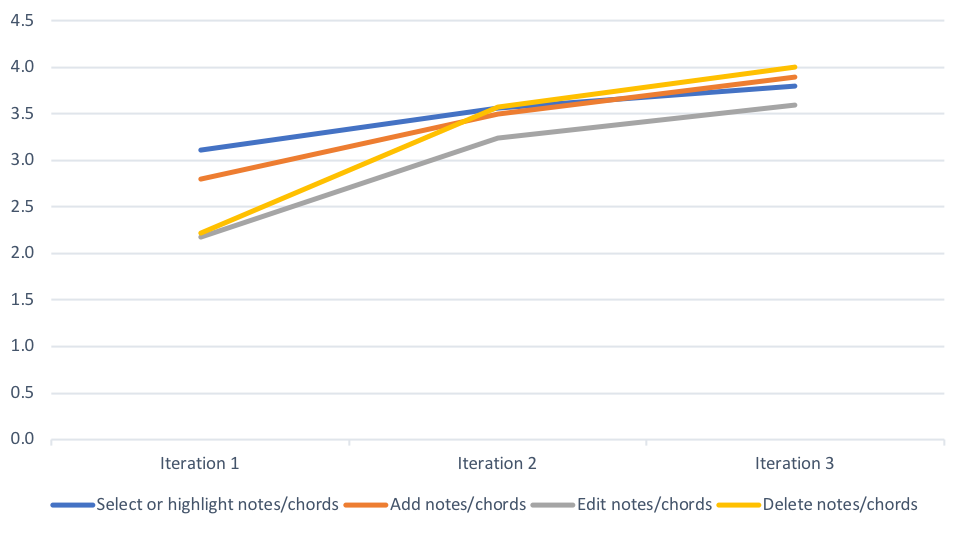
\includegraphics[scale=0.7]{figures/line-chart}}
		    \caption{Line chart showing the summarized common samples feature scores from iteration 1  - 3.}
		    \label{fig:common-samples-line}
		\end{figure} 

			\begin{comment}
				Cut, copy, or paste notes/chords & 4.0 & 4.0 & 3.0 & 4.0 & 3.5 & 3.7 & 3.0 & 4.0 & 0.4 \\ \hline
				Undo/redo an action & 3.5 & 4.0 & 4.0 & 4.0 & 4.0 & 3.9 & 3.5 & 4.0 & 0.2 \\ \hline
				Music Playback & 3.0 & 2.0 & 3.0 & 4.0 & 4.0 & 3.2 & 2.0 & 4.0 & 0.8 \\ \hline
				\end{comment}
	
	% section comparative_analysis (end)


